\documentclass[11pt]{article}
\usepackage[margin=0.85in]{geometry}
\usepackage{amsmath,amssymb,booktabs,array,tabularx,multirow}
\usepackage{tikz,pgfplots,units}
\usetikzlibrary{arrows.meta,patterns,positioning,decorations.pathreplacing}
\pgfplotsset{compat=1.18}

\newcommand{\FUNWAVE}{FUNWAVE--TVD}
\newcommand{\ie}{{\it i.e.,}~}

\setlength{\parindent}{0em}    % Set paragraph indentation (e.g., 2em, 1cm, or 15pt)
\setlength{\parskip}{0.5em}      % Set vertical spacing between paragraphs (e.g., 1ex or 6pt)


\title{FUNWAVE--TVD Rip-Channel Model Domain and Parameter Space}
\author{}
\date{Working configuration: \texttt{spreadRip}, \texttt{highRip}, \texttt{gapRip}, \texttt{highRip1}, and \texttt{gapRip1}}
\begin{document}
\maketitle

\section{Purpose and run organization}
This document summarizes the idealized bathymetry and wave-forcing parameter space generated by the MATLAB workflow for the rip-channel simulations currently under analysis.  A run family (e.g. \texttt{spreadRip}) selects a set of bathymetric grids and wave parameters.  Each permutation is encoded as
\begin{equation}
\texttt{hHHtTTsSSdDD},
\end{equation}
where \texttt{HH}/10 is $H_s$ [m], \texttt{TT} is $T_p$ [s], \texttt{SS} is directional spread [deg], and \texttt{DD} is peak direction [deg].  The grid name is prepended to this wave identifier when the run directory is constructed.

\section{Cross-shore domain}
\subsection{Background profile and flat region}
The cross-shore coordinate is $x$, with the nominal zero-depth intercept fixed at
\begin{equation}
 x_0=50~\mathrm{m}.
\end{equation}
All cases considered here use a background slope $s=0.03$ and grid
resolution of $\Delta x=0.5~\unit{m}$ and $\Delta y=1~\unit{m}$.
Before adding the bar/terrace feature, the depth is initialized as,
\begin{equation}
 h_p(x)=\min\left[s(x-x_0),h_{\rm flat}\right],\qquad h_{\rm flat}=9~\mathrm{m}.
\end{equation}
Thus the planar slope reaches the $9$-m offshore flat region after $h_{\rm
  flat}/s=300$ m, nominally at $x=350$ m.  The slope-to-flat
transition is smoothed with a normalized Hamming window whose width is
approximately one-half of the design wavelength (\ie $\lambda\approx 88~$m for $T=10~$s in $h=9~$m).


\begin{figure}[htbp]
\centering
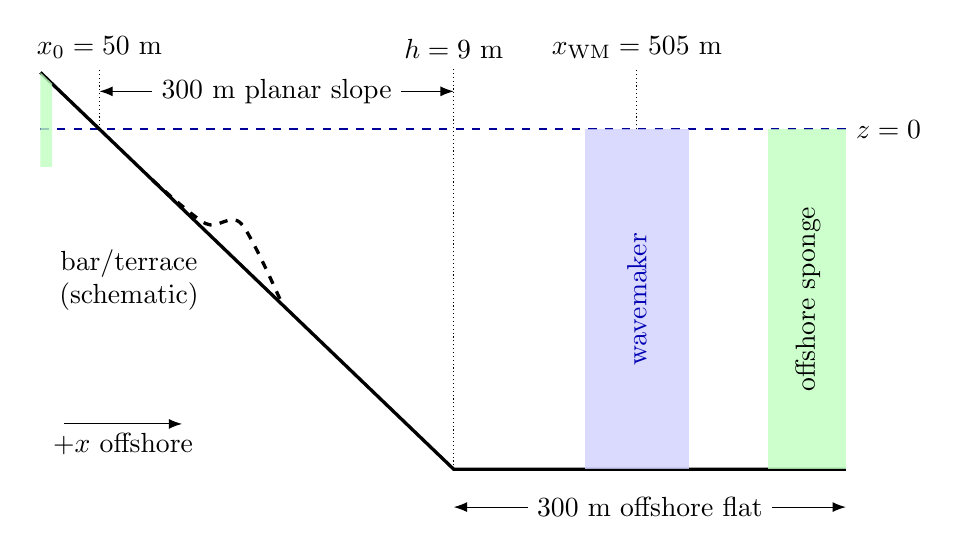
\begin{tikzpicture}[x=0.015cm,y=0.48cm,>=Latex]
  % water and bottom
  %\fill[cyan!8] (0,0) rectangle (682,-9.6);
  \draw[blue!60!black,dashed,thick] (0,0)--(682,0) node[right,black] {$z=0$};
  \draw[very thick] (0,1.5) -- (50,0) -- (350,-9) -- (682,-9);
  % schematic bar/terrace
  \draw[very thick,dashed] plot[smooth] coordinates {(95,-1.35) (140,-2.5) (170,-2.5) (205,-4.65)};
  \node[align=center,fill=white,inner sep=2pt] at (75,-4) {bar/terrace\\(schematic)};
  % wavemaker region
  \fill[blue!18,opacity=.8] (460.9,0) rectangle (549.1,-9);
  % \draw[blue!70!black,thick] (505,0)--(505,-9);
  \draw[densely dotted] (505,0)--(505,1.6) node[above] {$x_{\rm WM}=505$ m};  
  \node[rotate=90,blue!70!black] at (505,-4.5) {wavemaker};
  % sponges
  \fill[green!25,opacity=.8] (0,1.5) -- (10,1.2) -- (10,-1.0) -- (0,-1.0)--cycle;
  \fill[green!25,opacity=.8] (615.8,0) rectangle (682,-9);
  \node[rotate=90] at (650,-4.5) {offshore sponge};
%  \node[rotate=90] at (5,0.25) {shore sponge};
  % annotations
  \draw[<->] (50,1.0)--(350,1.0) node[midway,fill=white] {$300$ m planar slope};
  \draw[<->] (350,-10.0)--(682,-10.0) node[midway,fill=white] {$300$ m
    offshore flat};
  \draw[densely dotted] (50,0)--(50,1.6) node[above] {$x_0=50$ m};
  \draw[densely dotted] (350,-9)--(350,1.6) node[above] {$h=9$ m};
  \draw[->] (20,-7.8)--(120,-7.8) node[midway,below] {$+x$ offshore};
\end{tikzpicture}
\caption{Cross-shore model geometry.  The dashed nearshore curve is illustrative: the actual Gaussian feature differs between bar and terrace families as specified below.  The wavemaker shading represents the width $W$ used in bathymetry construction; FUNWAVE receives the wavemaker center $x_{\rm WM}$ and depth $h_{\rm WM}=9$ m.}
\label{fig:crossshore}
\end{figure}


\subsection{Wavemaker and sponge layers}

The wavemaker region is in $9~\unit{m}$ depth and the width is set to
one wavelength, $W_\mathrm{\rm WM}=\lambda$. Onshore and offshore of the wavemaker are
flat regions to allow the waves to adjust before approaching the slope
and sponge, resulting in a cross-shore domain width of $W_x\approx682$ m and
$x_{\rm WM}\approx505$ m. 

\emph{where should I discuss the waves simulated for the analysis?
  This section is just info pertinent to the grid...}


Offshore of the wavemaker, a $70\mbox{-}\unit{m}$
wide sponge layer is used to absorb incoming waves using a combination
of the Larson-Dansy 1983 direct sponge and a friction/drag type
sponge. To minimize wave reflections from the sponge layer,
one dimensional simulations were conducted with constant 9-m depth and varying free
parameters $\gamma_s$ in the L-D formulation and $C_\mathrm{sponge}$ in the
friction/drag forumulations. The simulation with smallest reflections
used $\gamma_s=0.8718$ and $C_\mathrm{sponge}=2.8844$, and these
values were used in all subsequent simulations.


% Preamble:
% \usepackage{tikz}
% \usepackage{pgfplots}
% \usepgfplotslibrary{groupplots}
% \pgfplotsset{compat=1.18}

\begin{figure}[htbp]
\centering
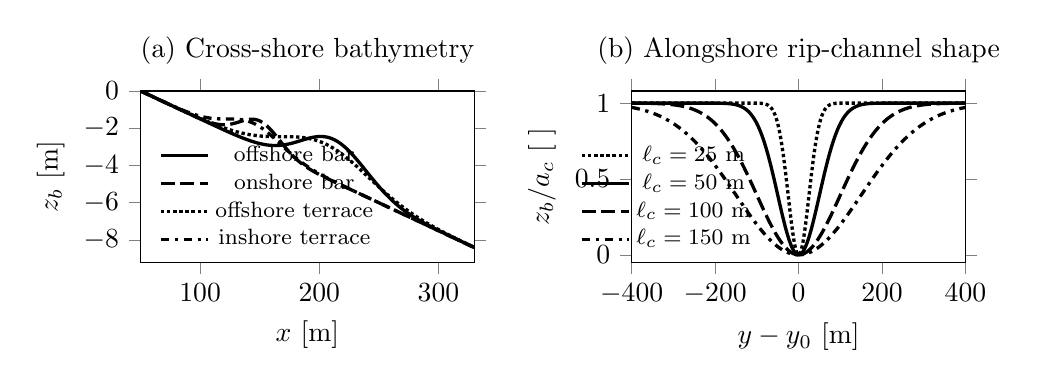
\begin{tikzpicture}

% ============================================================
% LEFT PANEL: cross-shore bar / terrace profiles
% ============================================================
\begin{axis}[
    name=crossshore,
    width=0.48\textwidth,
    height=0.31\textwidth,
    xmin=50, xmax=330,
    ymin=-9.2, ymax=0.0,
    xlabel={$x$ [m]},
    ylabel={$z_b$ [m]},
    title={(a) Cross-shore bathymetry},
    tick align=outside,
    axis line style={black},
    legend style={
        font=\footnotesize,
        draw=none,
        fill=none,
        at={(0.03,0.01)},
        anchor=south west,
        row sep=-1pt
    },
    samples=250,
    domain=50:330,
]

% Background planar beach: z_b = -0.03(x-50)
% \addplot[
%     black,
%     dashed,
%     thick
% ]
% {-0.03*(x-50)};
% \addlegendentry{planar}

% ------------------------------------------------------------
% Original Gaussian bar
% xc = 212 m, wc = 27.5 m, ac = 2.26 m
%
% h = s(x-x0) - a exp[-0.5((x-xc)/wc)^2]
% zb = -h
% ------------------------------------------------------------
\addplot[
    very thick
]
{-0.03*(x-50)
 + 2.26*exp(-0.5*((x-212)/27.5)^2)};
\addlegendentry{offshore bar}

% Shoreward / lower Gaussian bar ("bar1")
% xc = 150 m, wc = 16.83 m, ac = 1.39 m
\addplot[
    very thick,
    dash pattern=on 5pt off 2pt
]
{-0.03*(x-50)
 + 1.39*exp(-0.5*((x-150)/16.83)^2)};
\addlegendentry{onshore bar}

% ------------------------------------------------------------
% Original terrace
% xc = 205 m, wc = 36.6 m, ac = 1.81 m
% ------------------------------------------------------------
\addplot[
    very thick,
    densely dotted
]
{-0.03*(x-50)
 + 1.81*exp(-0.5*((x-205)/36.6)^2)};
\addlegendentry{offshore terrace}

% Shoreward / lower terrace ("ter1")
% xc = 145 m, ac = 1.11 m
%
% wc is calculated in the MATLAB code as
% round(100*ac/slope*exp(-1/2))/100
% = approximately 22.44 m
\addplot[
    very thick,
    dash dot
]
{-0.03*(x-50)
 + 1.11*exp(-0.5*((x-145)/22.44)^2)};
\addlegendentry{inshore terrace}

% % Mean sea level
% \addplot[
%     black,
%     thin,
%     forget plot
% ]
% coordinates {(50,0) (330,0)};

% \node[
%     anchor=south west,
%     font=\scriptsize
% ] at (axis cs:55,0.05) {$z=0$};

\end{axis}


% ============================================================
% RIGHT PANEL: alongshore Gaussian rip-channel shapes
%
% The MATLAB bathymetry uses
%
% bar(y) = bar_0 [
%       1 - r_c exp(-0.5((y-L_y/2)/l_c)^2)
% ]
%
% with rc = 1.
%
% Plot normalized remaining bar amplitude:
%
% B(y)/B_0 = 1 - exp[-0.5(y/l_c)^2].
%
% Thus B/B0 = 0 at the channel center and tends to 1 away
% from the rip.
% ============================================================
\begin{axis}[
    at={(crossshore.east)},
    anchor=west,
    xshift=2cm,
    width=0.48\textwidth,
    height=0.31\textwidth,
    xmin=-400, xmax=400,
    ymin=-0.05, ymax=1.08,
    xlabel={$y-y_0$ [m]},
    ylabel={$z_b/a_c$ [~]},
    title={(b) Alongshore rip-channel shape},
    tick align=outside,
    axis line style={black},
    legend style={
        font=\footnotesize,
        draw=none,
        fill=none,
        at={(0.4,0.01)},
        anchor=south east,
        row sep=-1pt
    },
    samples=250,
    domain=-400:400,
]

% Rip2: lc = 25 m
\addplot[
    very thick,
    densely dotted
]
{1-exp(-0.5*(x/25)^2)};
\addlegendentry{$\ell_c=25$ m}

% Rip1: lc = 50 m
\addplot[
    very thick
]
{1-exp(-0.5*(x/50)^2)};
\addlegendentry{$\ell_c=50$ m}

% Rip0: lc = 100 m
\addplot[
    very thick,
    dash pattern=on 5pt off 2pt
]
{1-exp(-0.5*(x/100)^2)};
\addlegendentry{$\ell_c=100$ m}

% Rip3: lc = 150 m
\addplot[
    very thick,
    dash dot
]
{1-exp(-0.5*(x/150)^2)};
\addlegendentry{$\ell_c=150$ m}

% % Channel center
% \addplot[
%     black,
%     thin,
%     dashed,
%     forget plot
% ]
% coordinates {(0,-0.05) (0,1.08)};

% \node[
%     anchor=south,
%     font=\scriptsize
% ] at (axis cs:0,0.02) {rip center};

\end{axis}

\end{tikzpicture}

\caption{
Idealized bathymetric variations used in the FUNWAVE-TVD
rip-channel simulations.
(a) Cross-shore profiles showing the common planar beach
(slope $s=0.03$) and the Gaussian bar and terrace perturbations.
The \texttt{bar1} and \texttt{terrace1} configurations are
shoreward, lower-amplitude variants of the original features.
(b) Alongshore structure of the rip channel, shown as the
normalized remaining bar/terrace amplitude for the four
Gaussian channel scales $\ell_c$.
}
\label{fig:ripchannel_geometry}
\end{figure}


\subsection{Bar and terrace profiles}
Barred and terraced profiles are created by subtracting the Gaussian profile,
\begin{equation}
 B(x)=a_c\exp\left[-\frac{1}{2}\left(\frac{x-x_c}{w_c}\right)^2\right],
\end{equation}
from the planar depth profile, $h=h_p-B$.  The parameter $a_c$
is the feature height above the planar background and $w_c$
is its cross-shore width.

The terraced profiles are a special case of $(a_c,w_c)$ where the slope $dh/dx$ is
zero at $(x-x_c)/w_c=-1$, for which,
\[w_c=\frac{a_c}{\beta}\exp{\left(-\frac{1}{2}\right)}.\]
One dimensional simulations on the planar slope were conducted to identify
the depth of breaking $h_{\rm br}$ for incident waves having a JONSWAP
frequency spectrum with $\gamma=3$, $T_p=10~$s, and
$H_\mathrm{s}= 0.5~$m and $1.0~$m. The outer/inner bar locations $x_c$
were chosen such that $h_p(x_c) \approx a_c+h_{\rm br}$, using
$a_c=0.75 h_{\rm br}$. The amplitude (width) of the barred profiles
are increased (decreased) by $25\%$ relative to terraced cases. The
resulting barred profile $w_c$ are approximately half
of the local peak wavelength $\lambda/2$, with water depths at the bar
crest approximately equal to $h_{\rm br}$. 


\begin{table}[htbp]
\centering
\caption{Cross-shore bathymetric feature definitions used by the analyzed run families.}
\begin{tabular}{llccc}
\toprule
Grid prefix & Feature family & $x_c$ [m] & $w_c$ [m] & $a_c$ [m]\\
\midrule
\texttt{barRip*}  & bar, original & 212 & 27.50 & 2.26\\
\texttt{terRip*}  & terrace, original & 205 & 36.60 & 1.81\\
\texttt{bar1Rip*} & bar, shoreward/lower & 150 & 16.83 & 1.39\\
\texttt{ter1Rip*} & terrace, shoreward/lower & 145 & 22.44 & 1.11\\
\bottomrule
\end{tabular}
\end{table}

\section{Alongshore domain and rip-channel geometry}
All two-dimensional rip-channel grids use $L_y=3000$ m, with periodic
alongshore boundaries.  The channel is centered at $y=L_y/2$ and
attenuates the Gaussian bar/terrace amplitude in $y$ following,
\begin{align}
 B(x,y) &= B(x)\left[1-r_c\exp\left(-\frac{1}{2}\left(\frac{y-L_y/2}{\ell_c}\right)^2\right)\right],\\
 h(x,y) &= h_p(x)-B(x,y),
\end{align}
where $r_c=1$ for the rip-channel grids analyzed here. Consequently,
the bar/terrace perturbation vanishes at the channel centerline.  The
parameter $\ell_c$ is the Gaussian alongshore scale and varied from
25m-150m (Figure~\ref{fig:ripchannel_geometry}b).

% \begin{figure}[htbp]
% \centering
% \begin{tikzpicture}[x=0.015cm,y=0.003cm,>=Latex]
%   \draw[thick] (0,0) rectangle (600,3000);
%   \fill[gray!18] (100,0) rectangle (260,3000);
%   \node[rotate=90] at (180,400) {bar/terrace zone};
%   % gaussian channel represented as widening white cut through feature
%   \fill[white] plot[smooth] coordinates {(100,1200) (130,1300) (180,1400) (250,1500) (180,1600) (130,1700) (100,1800)} -- (100,1200);
%   \draw[dashed,thick] (0,1500)--(600,1500) node[right] {$y=L_y/2$};
%   \draw[<->] (300,1500)--(300,1650) node[midway,right] {$\ell_c$ (schematic)};
%   \draw[->] (420,500)--(520,500) node[midway,below] {$+x$};
%   \draw[->] (420,500)--(420,900) node[midway,left] {$+y$};
%   \node[align=center] at (470,2350) {$L_y=3000$ m\\periodic in $y$};
% \end{tikzpicture}
% \caption{Plan-view schematic of the alongshore domain.  The white indentation represents Gaussian removal of the bar/terrace feature at the rip centerline, not a hard-edged channel.}
% \label{fig:alongshore}
% \end{figure}

The grid suffix maps to $\ell_c$ as
\begin{equation}
\texttt{Rip0}:100~\mathrm{m},\qquad
\texttt{Rip1}:50~\mathrm{m},\qquad
\texttt{Rip2}:25~\mathrm{m},\qquad
\texttt{Rip3}:150~\mathrm{m}.
\end{equation}
For intuition, the full width between the two $e^{-1/2}$ points is $2\ell_c$, while the Gaussian FWHM is $2\sqrt{2\ln2}\,\ell_c\approx2.355\ell_c$.  These are derived width measures; the model itself is parameterized by $\ell_c$.

\section{Analyzed parameter space}
All five run families use $T_p=10$ s and normally incident waves
($\theta_p=0^\circ$).  Their parameter combinations are summarized in
Table~\ref{tab:families}.  Each listed wave combination is crossed
with every listed grid in that family.

The irregular wavemaker option
\texttt{WK\_NEW\_IRR} is used, but the source code is modified to use
the maximum possible angular resolution at peak period by default and
remove wave components whose amplitude is below
$10^{-6}~\unit{m}$. When shifting directional wave components from a
regular grid to the nearest allowable mode, pairs of wave components
with the same alongshore mode and frequency difference
$f_i-f_j<0.25(f_{\rm max}-f_{\rm min}) N_{\rm \theta}/N_{\rm freq}$
are combined to conserve wave energy and reduce computational overhead.

\begin{table}[htbp]
\centering
\caption{Run-family matrix for the simulations currently being
  analyzed. ***Need to add missing gapRip-barRip0 to complete
  parameter space.}
\label{tab:families}
\small
\begin{tabularx}{\textwidth}{l c c c X}
\toprule
Family & $H_s$ [m] & $T_p$ [s] & Spread [deg] & Bathymetric grids\\
\midrule
\texttt{spreadRip} & 1.0 & 10 & 1, 2, 4, 10, 20 & \texttt{barRip1}, \texttt{terRip1}\\
\texttt{highRip}   & 1.5 & 10 & 1, 10 & \texttt{barRip1}, \texttt{terRip1}\\
\texttt{gapRip}    & 1.0 & 10 & 1, 10 & \texttt{barRip2}, \texttt{barRip3}, \texttt{terRip0}, \texttt{terRip2}, \texttt{terRip3}\\
\texttt{highRip1}  & 0.5, 1.0, 1.5 & 10 & 1, 10 & \texttt{bar1Rip1}, \texttt{ter1Rip1}\\
\texttt{gapRip1}   & 1.0 & 10 & 1, 10 & \texttt{bar1Rip0--3}, \texttt{ter1Rip0--3}\\
\bottomrule
\end{tabularx}
\end{table}

\begin{table}[htbp]
\centering
\caption{Bathymetry--rip-width matrix represented across the five run
  families. A check indicates that the grid occurs in at least one
  analyzed family. ***Need to add missing gapRip-barRip0 to fill matrix.}
\small
\begin{tabular}{llcccc}
\toprule
Cross-shore family & Grid generation & $\ell_c=25$ & $50$ & $100$ & $150$ m\\
\midrule
Bar     & original (\texttt{barRip*})  & $\checkmark$ & $\checkmark$ & -- & $\checkmark$\\
Terrace & original (\texttt{terRip*})  & $\checkmark$ & $\checkmark$ & $\checkmark$ & $\checkmark$\\
Bar     & shoreward/lower (\texttt{bar1Rip*}) & $\checkmark$ & $\checkmark$ & $\checkmark$ & $\checkmark$\\
Terrace & shoreward/lower (\texttt{ter1Rip*}) & $\checkmark$ & $\checkmark$ & $\checkmark$ & $\checkmark$\\
\bottomrule
\end{tabular}
\end{table}

The experiment therefore separates three principal controls: (i) cross-shore bathymetric morphology (bar versus terrace, including the shoreward/lower ``1'' variants), (ii) alongshore rip-channel scale $\ell_c$, and (iii) offshore wave forcing through $H_s$ and directional spread.  Peak period and mean direction are held fixed for the five analysis families considered here.

\section{Implementation notes}
The run builder forms every permutation of the selected heights, periods, directional spreads, and directions, then combines these wave cases with each requested grid.  Bathymetry and gauge files are generated once per grid name and referenced by the FUNWAVE input file.  For the two-dimensional cases, $\Delta x=0.5$ m and $\Delta y=1$ m.  The generated input passes the grid dimensions, bathymetry file, wavemaker location/depth, $H_s$, $T_p$, peak direction, directional spread, and gauge definitions to FUNWAVE before appending the common sample-input controls.


\end{document}
